% !TeX spellcheck = de_CH_frami

\section{Frequenzverhalten von MOS-Verstärkern (Kap. 11)}
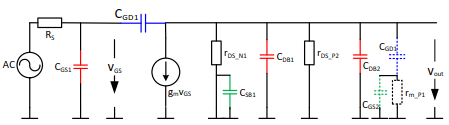
\includegraphics[width=0.5\linewidth]{chapters/Frequenzverhalten/images/parasitaere_kapazitaeten}
\textbf{Analyse mittels Open-Circuit Time Constant Methode} \\
Bestimmung des für die Bandbreite verantwortlichen Pols wie folgt:
\begin{compactenum}
	\item Setze alle unabhängigen Quellen = 0 (V => Kurzschluss, I => Leerlauf)
	\item Berechne für alle Kapazitäten die zugehörige Zeitkonstante, wenn alle anderen C = 0.
	\item Bestimme die Bandbreite als Summe der Zeitkonstanten: $\omega_{-3dB}\approx \frac{1}{\sum\tau_k}=\frac{1}{\sum R_kC_k}$
\end{compactenum}

